\documentclass[runningheads]{llncs}
\usepackage[T1]{fontenc}
\usepackage{graphicx}
\usepackage{booktabs}
\usepackage{amsmath,amssymb}
\usepackage{microtype}
\usepackage{url}
\usepackage{hyperref}
\hypersetup{hidelinks,hypertexnames=false}
\emergencystretch=1em
\usepackage{multirow}
\usepackage{float}
\usepackage{xspace}
\newcommand{\CN}{\textsc{CertiNeg}\xspace}
\newcommand{\FDP}{\operatorname{FDP}}
\newcommand{\ind}{\mathbb{I}}
\newcommand{\Prb}{\mathbb{P}}
\newcommand{\E}{\mathbb{E}}
\begin{document}
\raggedbottom
\title{Certified Absence: Design-Based Risk Control for Semantic \texttt{NOT EXISTS} Queries}
\titlerunning{Certified Absence for Semantic NOT EXISTS Queries}
\author{Anonymous Author(s)}
\authorrunning{Anonymous Author(s)}
\institute{Anonymous affiliation for the research draft}
\maketitle

\begin{abstract}
A grouped semantic \texttt{NOT EXISTS} query can return a false claim of absence after missing just one positive record. We formalize \emph{certified absence} as finite-population control of the group-level false-discovery proportion (FDP) of a frozen output set. \CN samples candidate groups without replacement, resolves sampled group truth exactly, and uses hypergeometric inversion with simultaneous or fixed-sequence multiple testing over predeclared nested outputs. Proxy scores determine inspection order; the guarantee does not require them to be calibrated. Exhaustive enumeration verifies coverage; a boundary case with true FDP $0.10083$ has exact false-certification probability $0.049745$ at $(\epsilon,\delta)=(0.10,0.05)$. On a controlled population, fixed-sequence certification retains 79.2\% versus 48.6\% for independent sample splitting. On SemBench Cars, a complete screen of 15 frequent complaint predicates exposes both certifiable and abstention regimes; four comparable nondegenerate workloads have 1,093--1,643 candidate groups and unsafe full-output FDPs of 14.6--16.9\%. Across five group-disjoint AIR BAGS splits, mean certified retention is $64.1\%\pm3.9\%$ with no unsafe return in 10,000 audit randomizations. Utility varies with grouping and risk targets. A frozen 0.6B-parameter LLM pilot produces no candidate absences, so certification cannot recover useful output from that executor.
\keywords{Semantic query processing \and LLM databases \and NOT EXISTS \and finite-population inference \and risk-limiting audits \and false discovery proportion}
\end{abstract}

\section{Introduction}
Query engines now use foundation models to evaluate predicates over structured and unstructured data. LOTUS formalizes these semantic operators~\cite{lotus2025}, and SemBench benchmarks engines that implement them~\cite{sembench2026}. Grouped negative queries arise naturally in this setting: a user might ask for camera-days with no image of a target species, cars with no indication of a safety issue in any modality, or customer accounts with no document satisfying a semantic condition.

These queries are vulnerable to missed positives. In a group with only one positive record, a single row-level false negative can cause the engine to report absence for the whole group. High record-level accuracy or recall therefore gives no direct answer to the user's question: what fraction of the returned groups actually contain a positive? We measure error at the returned-group level.

Evergreen already supports grouped semantic claim verification, witness stopping, finite-population sampling, confidence sequences, and multiplicity control~\cite{evergreen2026}; risk-limiting audits provide sequential and weighted finite-population tools~\cite{alpha2023,rlfa2023}. We use these established mechanisms to study the FDP of a frozen returned set of negative groups.

Let $A$ be the committed output of a semantic \texttt{NOT EXISTS} query. We ask whether the fraction of returned groups that secretly contain a positive record is at most $\epsilon$, with audit risk $\delta$. The guarantee concerns false discoveries across the returned set; per-claim scores and model posteriors answer different questions.

Our contributions are:
\begin{enumerate}
\item We formalize \emph{certified semantic absence} as a finite-population design-based guarantee on the group-level FDP of a frozen negative-query output.
\item We use probability-sampled outer groups and exact inner verification; proxies may reduce inspection cost but never enter validity.
\item We combine exact hypergeometric testing with simultaneous or fixed-sequence selection over predeclared nested outputs, and characterize exact-negative cost including the near-census burden at $\epsilon=0$.
\item We provide exhaustive tests and controlled/SemBench experiments covering tightness, baselines, audit budget, family granularity, target sensitivity, predicate screening, split/ranking robustness, alternative grouping, and a frozen small-LLM pilot.
\end{enumerate}


\section{Background and Related Work}
\subsection{Semantic query processing}
LOTUS provides declarative semantic operators~\cite{lotus2025}, and SemBench benchmarks semantic query engines~\cite{sembench2026}. \CN operates after such an execution layer freezes a negative candidate set.

SUPG certifies proxy-assisted precision/recall~\cite{supg2020}, BARGAIN provides guarantees for LLM cascades~\cite{bargain2026}, and Semantic Views certifies semantic-filter precision/recall from fresh oracle samples~\cite{semviews2026}. For nonempty outputs, our FDP equals one minus precision when each group is treated as a unit with label $1-Z_g$. Thus grouped-absence certification can use precision-control tools at the group level. Obtaining exact group labels is the operational difficulty. One positive witness refutes absence, but confirming absence requires checking every record. Our study concerns the resulting selection and cost trade-off; the generic precision guarantee is already available. Run-to-run query variation motivates freezing the candidate output before audit~\cite{variance2026}.

\subsection{Claim verification versus output-set certification}
Evergreen is the closest systems work~\cite{evergreen2026}: it verifies cardinal, proportional, and grouped semantic claims using witness stopping, finite-population sampling, confidence sequences, and multiplicity control.

We estimate FDP across the returned negative set and resolve each audited group's truth exactly. The semantic proxy affects inspection cost while the outer confidence bound uses only audited group labels. Selection is restricted to a predeclared nested family. Confidence sequences, multiplicity correction, and witness-first ordering are established tools.

\subsection{Finite-population and prediction-assisted inference}
Sampling without replacement provides the finite-population basis~\cite{cochran1977}; risk-limiting audits add sequential and weighted tools~\cite{alpha2023,rlfa2023}. Learn-then-Test develops fixed-sequence calibration~\cite{ltt2025}; conformal selection controls false selections under exchangeability~\cite{jin2023}. Our guarantee conditions on one fixed corpus. Its only randomness comes from the audit design, so it bounds output-set FDP for that corpus without a model-distribution guarantee.

\section{Problem Formulation}
Consider fixed groups $g=1,\ldots,G$. Group $g$ has records $i=1,\ldots,m_g$ and trusted binary reference labels
\begin{equation}
y_{gi}\in\{0,1\}.
\end{equation}
The group-level existential truth is
\begin{equation}
Z_g=\ind\{\exists i: y_{gi}=1\}.
\end{equation}
A semantic query engine predicts record-level predicate values and returns groups believed to satisfy \texttt{NOT EXISTS}. The engine may be an LLM, VLM, cascade, learned decision model, or other semantic operator. It produces a candidate set $A_0$ that is frozen before trusted audit labels are exposed.

For any nonempty $A\subseteq A_0$, define the group-level false-discovery proportion
\begin{equation}
\FDP(A)=\frac{\sum_{g\in A} Z_g}{|A|},
\label{eq:fdp}
\end{equation}
with $\FDP(\emptyset)=0$. A group counted by the numerator is a \emph{false absence}: the query reported no positive record, although at least one trusted positive exists in the recorded group.

Our target is
\begin{equation}
\Prb_{\mathrm{audit}}\!\left(\FDP(A_{\widehat{k}})>\epsilon\right)\le\delta,
\label{eq:target}
\end{equation}
where all records, labels, semantic outputs, and candidate sets are fixed, and probability is solely over randomized audit sampling. Equation~\eqref{eq:target} is a design-based statement about the finite corpus and its reference labels. It supplies neither a Bayesian posterior nor a claim about unrecorded real-world events.

We allow a predeclared nested family
\begin{equation}
A_1\subset A_2\subset\cdots\subset A_K=A_0,
\label{eq:nested}
\end{equation}
usually constructed before the audit by sorting candidate groups by a model risk score and choosing fixed retention fractions. The score need not be calibrated for the guarantee developed below.

\section{CertiNeg}
\begin{figure}[t]
\centering
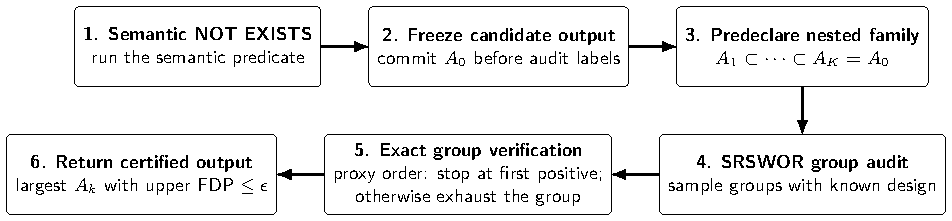
\includegraphics[width=\linewidth]{../figures/architecture.pdf}
\caption{\CN separates semantic execution from certification. The semantic output and the nested candidate family are committed before trusted labels are revealed. A probability sample of groups is then resolved exactly, using a proxy only to order records inside each audited group.}
\label{fig:arch}
\end{figure}

\subsection{Freeze first, audit second}
Before any audit label is requested, the implementation commits the data snapshot, query, semantic plan, model identifiers, prompts/decoding settings, candidate groups, risk scores, and code version. A production artifact can record these commitments as hashes in a \texttt{candidate\_groups.jsonl} manifest. The query and threshold must then remain fixed when audit evidence arrives. Documented run-to-run variation in semantic queries makes this commitment necessary~\cite{variance2026}.

\subsection{Exact inner group verification}
For an audited group $g$, let $s_{gi}$ be any proxy score available without revealing the trusted label. Inspect records in decreasing $s_{gi}$. If a positive witness is found at rank $r$, then $Z_g=1$ and inspection stops. If no witness is found, the group is declared $Z_g=0$ only after every record has been checked. Thus the trusted-label cost is
\begin{equation}
C_g=\begin{cases}
\min_{i:y_{gi}=1}\operatorname{rank}_s(i), & Z_g=1,\\
m_g, & Z_g=0.
\end{cases}
\label{eq:innercost}
\end{equation}
The ordering can come from the same semantic model, a cheaper encoder, a heuristic, or even random order. It changes $C_g$ but not the resolved $Z_g$.

\begin{proposition}[No-free-negative principle]
Suppose no assumption is imposed on labels of uninspected records. After inspecting a strict subset of records in a group and observing only zeros, the group truth $Z_g$ cannot be determined exactly.
\end{proposition}
\begin{proof}
Let record $j$ be uninspected. Two completions of the observed data are compatible with all evidence: one sets every uninspected label to zero, giving $Z_g=0$; the other sets $y_{gj}=1$, giving $Z_g=1$. Any deterministic declaration of exact negative truth is wrong under one completion. Therefore exact declaration of $Z_g=0$ requires exhausting the group unless additional modeling or assumptions are introduced. \qed
\end{proof}

A positive witness allows early stopping; a clean group requires a complete scan. Large clean groups can therefore dominate audit cost.

\subsection{Fixed-set finite-population certificate}
Let a fixed candidate set $A$ contain $N$ groups and an unknown total
\begin{equation}
M=\sum_{g\in A}Z_g.
\end{equation}
Draw $n$ groups by simple random sampling without replacement (SRSWOR), resolve their $Z_g$ values exactly, and observe $X=x$ defective groups. Conditional on the fixed population,
\begin{equation}
X\sim\mathrm{Hypergeom}(N,M,n).
\end{equation}
For significance level $\alpha$, define the upper confidence count
\begin{equation}
M_U(x)=\max\left\{m:\Prb_{M=m}(X\le x)>\alpha\right\},
\label{eq:hyperupper}
\end{equation}
where infeasible $m$ values are omitted. Set $U=M_U/N$ and certify $A$ whenever $U\le\epsilon$.

\begin{theorem}[Fixed-set certificate]
For a fixed set $A$ and SRSWOR audit as above,
\begin{equation}
\Prb_{\mathrm{audit}}\!\left(\FDP(A)>U\right)\le\alpha.
\end{equation}
Consequently, returning $A$ only when $U\le\epsilon$ has false-certification probability at most $\alpha$.
\end{theorem}
\begin{proof}
For a fixed true $M$, the lower-tail probability $p_M(X)=\Prb_M(X'\le X)$ is a valid discrete $p$-value for testing a population with $M$ defects against smaller observed defect counts. Hence $\Prb_M(p_M(X)\le\alpha)\le\alpha$. By construction, $M_U(X)<M$ exactly when the true $M$ is excluded by this lower-tail test. Therefore $\Prb(M>M_U)\le\alpha$, and division by fixed $N$ yields the result. \qed
\end{proof}

\subsection{Simultaneous post-selection among nested outputs}
To reuse audit labels across thresholds, draw one SRSWOR sample $S$ of size $n$ from the largest predeclared set $A_K$. For each $A_k$, define $S_k=S\cap A_k$, $n_k=|S_k|$, and $x_k=\sum_{g\in S_k}Z_g$. Conditional on the random $n_k$, symmetry of SRSWOR implies that $S_k$ is itself an SRSWOR sample of size $n_k$ from the fixed $A_k$.

Compute $U_k$ from Eq.~\eqref{eq:hyperupper} at level $\alpha=\delta/K$ (set $U_k=1$ if $n_k=0$), and choose
\begin{equation}
\widehat{k}=\max\{k: U_k\le\epsilon\},
\label{eq:khat}
\end{equation}
returning the empty set if no candidate certifies.

\begin{theorem}[Nested post-selection guarantee]
If the nested family in Eq.~\eqref{eq:nested} is fixed before audit labels are observed and $S$ is SRSWOR from $A_K$, then the selection rule in Eq.~\eqref{eq:khat} satisfies Eq.~\eqref{eq:target}.
\end{theorem}
\begin{proof}
For each $k$, conditional on any realized $n_k$, the fixed-set theorem gives $\Prb(\FDP(A_k)>U_k\mid n_k)\le\delta/K$. Averaging over $n_k$ preserves that bound. A union bound gives simultaneous coverage $\Prb(\exists k:\FDP(A_k)>U_k)\le\delta$. On the complementary event, any selected set with $U_{\widehat{k}}\le\epsilon$ has $\FDP(A_{\widehat{k}})\le U_{\widehat{k}}\le\epsilon$. \qed
\end{proof}

Bonferroni permits selection among all individually passing members, including a later threshold after an earlier failure, at the cost of conservative bounds. Weighted Bonferroni can preallocate unequal levels $\alpha_k$ with $\sum_k\alpha_k\le\delta$; this remains simultaneous but shifts power toward predeclared high-utility thresholds.

\subsection{Ordered fixed-sequence selection}
If the application accepts only the largest \emph{consecutively} certified prefix, standard fixed-sequence testing~\cite{ltt2025} avoids the $\delta/K$ penalty. Test $A_1,\ldots,A_K$ at level $\delta$ in the predeclared order, stop at the first $U_k>\epsilon$, and return the last passing set.

\begin{theorem}[Ordered fixed-sequence guarantee]
The fixed-sequence rule above satisfies Eq.~\eqref{eq:target}.
\end{theorem}
\begin{proof}
If every $A_k$ is safe, the violation event is empty. Otherwise let $j$ be the first index with $\FDP(A_j)>\epsilon$. Returning any unsafe set requires the procedure to reach $j$ and falsely certify $A_j$. The latter event is contained in the level-$\delta$ false-certification event of the fixed-set test for $A_j$, whose probability is at most $\delta$. Dependence among tests does not enlarge this event. \qed
\end{proof}
We use fixed-sequence testing by default when consecutive certification is acceptable. Simultaneous protection allows the auditor to skip a failed intermediate threshold. Sequential e-process and weighted audit constructions can improve other operating points~\cite{alpha2023,rlfa2023}.

\subsection{Why zero tolerated FDP is expensive}
Certifying $\epsilon=0$ requires ruling out even one defective group. Suppose an SRSWOR audit of $N$ candidate groups observes $x=0$ defects. To exclude the alternative $M=1$ at risk $\delta$, the probability of missing the unique defect must be at most $\delta$:
\begin{equation}
\Prb_{M=1}(X=0)=\frac{N-n}{N}\le\delta.
\end{equation}
Thus $n\ge (1-\delta)N$ (up to integer rounding) is necessary for the exact fixed-set construction to return an upper count of zero after observing no defects. At $\delta=0.05$, roughly 95\% of groups must be audited; at $\delta=0.01$, roughly 99\%. These near-census requirements apply before accounting for record inspections within each sampled group.

\section{Prototype and Reproducibility}
The prototype is implemented in Python with NumPy and SciPy. The core confidence routine inverts the hypergeometric CDF by monotone binary search. One sampled group set from $A_K$ can feed equal- or weighted-Bonferroni simultaneous bounds, or the ordered fixed-sequence rule. No model probability enters the confidence calculation.

Our reproducibility package contains code, exhaustive validity tests, frozen experiment inputs, machine-readable results, and figure scripts with fixed seeds. A production interface should additionally persist an immutable candidate manifest and replayable audit trace.

\section{Experimental Methodology}
\subsection{Research questions}
We examine exact coverage (RQ1), the mismatch between row and group errors (RQ2), selection utility against valid baselines (RQ3), audit cost and family granularity (RQ4), and sensitivity to predicates, splits, ranking and risk targets (RQ5).


\subsection{Controlled populations}
For RQ1, we exhaustively enumerate all defect counts and all possible sample outcomes for every $N\le30$, every $0\le n\le N$, and $\alpha\in\{0.10,0.05,0.01\}$. We also save a larger sparse grid through $N=40$.

For RQ2, we generate 1,500 groups with heavy-tailed sizes, mark 62\% as containing at least one positive, and simulate a semantic row predicate with target positive-row recall 0.92 and false-positive probability 0.002. A group enters the predicted-absence output only if no row is predicted positive. This simulation illustrates the error mechanism; it does not measure a particular LLM.

For RQ3--RQ5, we freeze a candidate population of 1,200 groups. Group sizes follow a clipped log-normal distribution (median 25, 95th percentile 138). Defect probability is correlated with a latent risk variable; candidate risk scores are noisy versions of that variable. Positive groups contain one to four positive records. Five predeclared sets retain 30, 45, 60, 80, and 100\% of candidates, with realized FDPs 0.0417, 0.0500, 0.0653, 0.0781, and 0.1158. The main comparison samples 800 groups and repeats 2,000 audits at $\delta=0.05$. We additionally sweep audit fractions 5, 10, 20, 35, 50, and 66.7\%. Family-granularity ablations use \emph{uniformly spaced} 30--100\% grids with $K\in\{5,10,20,50\}$; their $K=5$ grid (30/47.5/65/82.5/100\%) is intentionally different from the original 30/45/60/80/100\% family used in the main tables.

\paragraph{SemBench text workloads.} We use the public SemBench Cars complaint table and car metadata~\cite{sembench_repo}. A group-disjoint 65/35 split uses country, year, and fuel type as the grouping key. We first fit the same 20k-feature TF--IDF/logistic-loss SGD pipeline for the 15 most frequent training-set component classes and report the \emph{complete} screen in Table~\ref{tab:predicate-screen}. For comparable primary audits we then use the four screened cases with at least 1,000 candidate groups, unsafe full output at $\epsilon=0.10$, and a safe 80\% coarse prefix. These cases are selected for descriptive comparison. We report all screening outcomes to make that selection explicit. Each threshold is fixed from training positives before held-out evaluation. Candidate groups contain no predicted-positive complaint and are ordered by maximum semantic score; trusted labels are held-out \texttt{component\_class} values. Primary predicates audit approximately 35\% of candidates for 2,000 randomizations at $(\epsilon,\delta)=(0.10,0.05)$. AIR BAGS additionally repeats the full split--fit--audit pipeline for five fixed seeds and, on the primary split, sweeps audit budget, family size, risk ranking, and $\epsilon\in\{0.05,0.10,0.20\}$ with $\delta\in\{0.01,0.05,0.10\}$.

We hold semantic execution fixed across audit repetitions, as required by Eq.~\eqref{eq:target}. Run-to-run LLM variance~\cite{variance2026} is outside this probability statement.

\subsection{Metrics}
The primary validity metric is the empirical false-certificate frequency
\begin{equation}
\widehat v=\frac{1}{R}\sum_{r=1}^{R}\ind\{\FDP(A_{\widehat{k}_r})>\epsilon\}.
\end{equation}
We report an exact one-sided 95\% Clopper--Pearson upper bound on $v$. Utility is the selected fraction of $A_K$. As an unattainable reference, the \emph{oracle prefix} is the largest prefix in the frozen risk order whose true FDP is at most $\epsilon$. Audit cost is the number of trusted record labels inspected, including full exhaustion of sampled negative groups. If fixed proxy ordering makes exact group costs $c_g$ and $S$ is an $n$-group SRSWOR from $N$ candidates, then
\begin{equation}
\frac{\E[\sum_{g\in S}c_g]}{\sum_{g=1}^{N}c_g}=\frac{n}{N},
\label{eq:census-cost}
\end{equation}
so the group-audit fraction is also the design-expected trusted-label fraction of an exact census. We additionally compare proxy ordered inner inspection with random inner ordering.

\paragraph{Audit planning.} For a prospective target set of size $N_k$, fix a design FDP $q_0<\epsilon$ (from domain requirements or a separate pilot) and $M_0=\lfloor q_0N_k\rfloor$. For each candidate $n_k$, exact power is the Hypergeom$(N_k,M_0,n_k)$ probability mass over outcomes $x$ whose upper bound satisfies $U(N_k,n_k,x,\delta)\le\epsilon$; choose the smallest $n_k$ reaching the desired power $1-\beta$. With one outer SRSWOR sample from $A_K$, $\E[n_k]=nN_k/N_K$ gives an initial outer budget. For example, an 874-group target with $q_0=.07$, $(\epsilon,\delta)=(.10,.05)$, and 80\% desired power needs $n_k=334$ direct target-group audits. Planning values must be fixed before confirmatory labels are reused for certification.

\section{Results}
\subsection{Exact coverage and zero-FDP burden}
The exhaustive unit test found no undercoverage. Across every $N\le30$ and every sample size, the minimum coverages were 0.9000, 0.9500, and 0.9900 for nominal levels 0.90, 0.95, and 0.99 respectively. A boundary calculation also shows the fixed-set test need not be very conservative: at $N=1200$, $n=800$, $M=121$ (true FDP $0.10083$), $\epsilon=0.10$, and $\delta=0.05$, exact hypergeometric summation gives false-certification probability $0.049745$. The test can therefore operate close to its nominal risk even though the frozen experiments below record zero violations.

For zero tolerated FDP, the exact calculation requires near-census sampling: for $N=1000$, observing zero defects requires $n=900,950,990$ at $\delta=0.10,0.05,0.01$, respectively; the artifact tabulates the same integer-rounded result for $N\in\{50,100,500,1000\}$. A semantic confidence score alone cannot reduce this sampling requirement.

\subsection{Row accuracy does not answer the group question}
The controlled row-predicate experiment attained positive-row recall 0.9176. It returned 586 candidate-absence groups, of which 0.1024 contained at least one positive record. This simulated result shows how high row recall can coexist with substantial error in the returned set. It does not estimate group FDP for a production semantic engine. With existential semantics, the number and dependence of positives within each group matter.

\subsection{Controlled selected-set certification}
The ordered fixed-sequence policy retains 0.792 on average (median 0.80) on the frozen population. The full candidate set has true FDP 0.1158 and violates $\epsilon=0.10$, whereas the 80\% prefix has FDP 0.0781. No unsafe set was returned in 2,000 repetitions; the one-sided 95\% Clopper--Pearson upper bound on the empirical violation frequency is 0.00150. These repetitions test the procedure on the frozen population. Equation~\eqref{eq:target} remains the guarantee; the boundary calculation above checks near-nominal type-I behavior of the fixed-set test.



The 80\% set was selected in 96.0\% of audits and the 60\% set in 4.0\%; no audit returned the unsafe 100\% set. The fixed-sequence rule can therefore exploit the predeclared order without dividing $\delta$ by $K$.

\subsection{Stronger selection baselines}
Table~\ref{tab:baselines} compares selection rules at the same $(\epsilon,\delta)$ target. All one-sample methods use the identical 800-group SRSWOR sample. Equal simultaneous Bonferroni is the original fully simultaneous rule; retention-weighted simultaneous protection allocates $\alpha_k\propto |A_k|$ before seeing audit labels; ordered fixed-sequence testing uses level $\delta$ at each threshold and stops at the first failure. Independent sample splitting uses 500 groups to select a threshold and another 500 to certify it, auditing about 791 unique groups on average. A predeclared fixed 80\% output, tested from the identical outer sample without post-selection, retains 76.8\%. Fixed-sequence retains 79.2\%; this comparison isolates selection from simply testing a favorable fixed prefix.

\begin{table}[H]
\centering
\small
\caption{Audit-policy comparison on the frozen population; $R=2000$, $\epsilon=0.10$, $\delta=0.05$. Cost is proxy ordered trusted labels relative to an exact census.}
\label{tab:baselines}
\begin{tabular}{l r r r r}
\toprule
Method & Ret. & Groups & Census cost & Viol.\\
\midrule
Independent sample split & 0.486 & 791.3 & 66.0\% & 0\\
Equal simultaneous & 0.766 & 800.0 & 66.6\% & 0\\
Fixed 80\% output & 0.768 & 800.0 & 66.6\% & 0\\
Retention-weighted simultaneous & 0.770 & 800.0 & 66.6\% & 0\\
Fixed-sequence ordered & \textbf{0.792} & 800.0 & 66.6\% & 0\\
\bottomrule
\end{tabular}
\end{table}

\subsection{Audit budget, oracle gap, and family granularity}
Certified retention increases with the audit budget (Fig.~\ref{fig:budget}). With the original five-set family, controlled mean retention rises from 0.113 at a 10\% audit to 0.621 at 35\% and 0.792 at 66.7\%; AIR BAGS rises from 0.142 to 0.630 and 0.749 over approximately the same audit fractions. The corresponding $K=5$ oracle ceilings are 0.800 for both workloads, while the largest safe prefixes in the full frozen risk orders are 0.954 and 0.862. Thus the main controlled operating point nearly saturates its coarse family, whereas SemBench retains a visible statistical-power gap even before accounting for grid coarseness.

\begin{figure}[H]
\centering
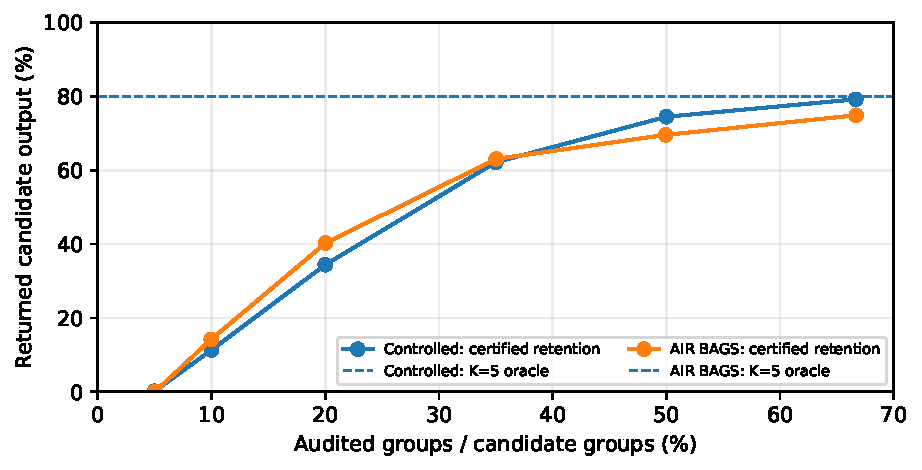
\includegraphics[width=.84\linewidth]{../figures/retention_budget.pdf}
\caption{Certified retention versus SRSWOR audit fraction. Dashed lines are the true-label oracle ceilings for the same five predeclared prefixes; they are references, not available to the algorithm. By Eq.~\eqref{eq:census-cost}, the horizontal axis also equals design-expected trusted-label cost relative to exact census.}
\label{fig:budget}
\end{figure}

Finer fixed-sequence grids allow more output sizes, but each additional test can stop the sequence. This ablation uses equally spaced 30--100\% grids: its $K=5$ row differs from the original family and is not directly comparable to the main tables. On the controlled population at the 800-group budget, uniform-grid mean retention rises from 0.790 ($K=5$) to 0.836, 0.856, and 0.867 for $K=10,20,50$; the continuous oracle is 0.954. For AIR BAGS at $n=383$, the corresponding means are 0.656, 0.701, 0.716, and 0.723 versus oracle 0.862. The empirical unsafe-return rates at $K=50$ are 2.2\% and 2.4\%, respectively (one-sided 95\% upper bounds 2.82\% and 3.04\%), consistent with but not replacing the 5\% design guarantee. Denser families can thus improve retention while also creating more opportunities to stop early, even without a Bonferroni correction.''

\subsection{Proxy and risk-ranking sensitivity}
The witness-first proxy reduces record inspections but cannot remove the cost of exhausting true negatives. At the main controlled operating point, proxy ordering saves 4.73\% relative to random inner order while the audit still consumes 66.6\% of exact-census labels; on AIR BAGS the corresponding values are 7.45\% and 35.0\%. The census ratios follow from SRSWOR in expectation (Eq.~\eqref{eq:census-cost}); the 65\% reduction on AIR BAGS comes from auditing a subset of groups, independently of the proxy's inspection-order savings.

Group-risk scores determine which prefixes are useful; validity holds for any frozen ranking. On AIR BAGS at a 35\% audit, the original semantic ordering retains 0.630 on average. Adding Gaussian score noise with standard deviation equal to one or three empirical score standard deviations reduces retention to $0.347\pm0.087$ and $0.017\pm0.028$ across ten frozen noisy rankings; fully random rankings retain essentially zero. A weak proxy can therefore leave little useful output to certify even though the audit guarantee still holds.

\section{End-to-End SemBench Workloads}
Table~\ref{tab:predicate-screen} reports every top-15 predicate tested under the same primary split and an approximately 35\% fixed-sequence audit. The four starred rows satisfy the stated operational filter ($N\ge1000$, full-output FDP $>0.10$, and a safe 80\% coarse prefix), but all outcomes are retained. For rows with $O_5=0$, any nonempty certificate is necessarily unsafe; their observed unsafe-return rates remain below the 5\% design target.

\begin{table}[H]
\centering
\scriptsize
\caption{Complete top-15 screen and fixed-sequence audits ($R=2000$, $\epsilon=.10$, $\delta=.05$, about 35\% audit). Each half reports candidate count $N$, true FDP, coarse oracle $O_5$, nonempty-certificate rate / mean retention (C/R), and unsafe-return rate U. Stars mark the four primary workloads.}
\label{tab:predicate-screen}
\setlength{\tabcolsep}{2pt}
\begin{tabular}{@{}lrrrrr@{\hspace{3pt}}lrrrrr@{}}
\toprule
Predicate & $N$ & FDP & $O_5$ & C/R & U\% & Predicate & $N$ & FDP & $O_5$ & C/R & U\%\\
\midrule
Electrical & 5 & 1.00 & .00 & 0/.000 & 0 & Veh. speed & 820 & .324 & .00 & 0/.000 & 0\\
Power train & 17 & .471 & .00 & 0/.000 & 0 & VIS./WIPER$^*$ & 1428 & .169 & .80 & 100/.708 & 0\\
Engine & 31 & .452 & .00 & 0/.000 & 0 & Fuel/prop. & 1368 & .249 & .00 & .15/.000 & .15\\
Steering & 376 & .287 & .00 & 0/.000 & 0 & Fwd. coll. & 1378 & .229 & .30 & 35/.108 & 2.15\\
Service br. & 431 & .339 & .00 & .65/.002 & .65 & EXT. LIGHT.$^*$ & 1643 & .146 & .80 & 100/.789 & 0\\
Structure & 932 & .275 & .00 & .10/.000 & .10 & Fuel system & 1693 & .093 & 1.00 & 100/.835 & 0\\
AIR BAGS$^*$ & 1093 & .155 & .80 & 96/.630 & 0 & Suspension & 1690 & .192 & .30 & 10.9/.036 & 2.15\\
ENG.+COOL.$^*$ & 1100 & .146 & .80 & 97.2/.549 & 0 & & & & & &\\
\bottomrule
\end{tabular}
\end{table}
\setlength{\tabcolsep}{6pt}


ENGINE AND ENGINE COOLING is abbreviated as ENGINE+COOLING. Depending on the predicate, the audit abstains, certifies part of the output, or starts with a full output that is already safe. Table~\ref{tab:sembench-real} details the four primary workloads.

\begin{table}[H]
\caption{Held-out SemBench Cars predicates on the primary split; target $(\epsilon,\delta)=(0.10,0.05)$, $R=2000$, and approximately 35\% of candidate groups audited. ``Oracle'' is the largest safe member of the fixed 30/45/60/80/100\% family.}
\label{tab:sembench-real}
\centering
\small
\begin{tabular}{lrrrrr}
\toprule
Predicate & F1 & Groups & Cand. FDP & Oracle & Retention $\pm$ SD \\
\midrule
AIR BAGS & .826 & 1093 & .155 & .800 & $.630\pm.160$\\
ENGINE+COOLING & .787 & 1100 & .146 & .800 & $.549\pm.138$\\
VIS./WIPER & .764 & 1428 & .169 & .800 & $.708\pm.100$\\
EXT. LIGHTING & .724 & 1643 & .146 & .800 & $.789\pm.045$\\
\bottomrule
\end{tabular}
\end{table}

For AIR BAGS, we also repeat the experiment across splits. Across five fixed group-disjoint 65/35 splits, record-level F1 is $0.826\pm0.007$, candidate FDP is $0.161\pm0.007$, and split-level mean certified retention is $0.641\pm0.039$ at the approximately 35\% audit budget. The standard deviation here is across the five split-level means; within each split there is additional audit-randomization variability. No unsafe output is returned in any of the five splits (2,000 audit randomizations each; per-split one-sided 95\% upper bound 0.00150).

\paragraph{Risk-target sensitivity.} Table~\ref{tab:epsdelta} varies the user-facing tolerance $\epsilon$ and audit risk $\delta$ while holding the primary AIR BAGS split, 35\% audit, fixed five-set family, and 2,000 SRSWOR draws fixed. Stricter targets sharply reduce utility, whereas $\epsilon=0.20$ makes the full output truly safe and is usually certified. No unsafe return occurs in any of the 18,000 sweep runs; the design guarantee applies independently of these empirical counts.

\begin{table}[H]
\centering
\small
\caption{AIR BAGS mean certified retention under $(\epsilon,\delta)$ sensitivity at $n=383$ ($R=2000$ per cell). Oracle is the largest truly safe member of the original five-set family.}
\label{tab:epsdelta}
\begin{tabular}{lrrrr}
\toprule
$\epsilon$ & $\delta=.01$ & $\delta=.05$ & $\delta=.10$ & Oracle\\
\midrule
.05 & .019 & .076 & .135 & .600\\
.10 & .491 & .630 & .678 & .800\\
.20 & .930 & .971 & .988 & 1.000\\
\bottomrule
\end{tabular}
\end{table}

\subsection{Alternative grouping under a parent-disjoint split}
An additional experiment splits on (country, year), seed 20261026, so both fuel-type and transmission groups remain disjoint between training and evaluation. The original experiments retain their original splits. Table~\ref{tab:grouping} holds row predictions and training-positive thresholds fixed while changing the grouping key. Transmission groups have higher candidate FDP and lower certified retention. At approximately two-thirds audit, their retention becomes .448, .144, .452 and .452 in table order. Across both budgets the largest per-configuration one-sided 95\% upper bound on unsafe-return frequency is .0332; these diagnostics do not replace the design guarantee.

\begin{table}[H]
\centering\small
\caption{Grouping sensitivity at about 35\% audit; 2,000 repetitions per cell. F/T denote fuel-type/transmission groups, each also keyed by country and year. U is the number of unsafe returns for T (zero for F).}
\label{tab:grouping}
\begin{tabular}{lrrrr}
\toprule
Predicate & Groups F/T & FDP F/T & Retention F/T & U\\
\midrule
AIR BAGS & 1086/388 & .161/.284 & .661/.201 & 11\\
ENGINE+COOLING & 1134/385 & .143/.205 & .586/.049 & 32\\
VIS./WIPER & 1416/587 & .150/.266 & .792/.205 & 0\\
EXT. LIGHTING & 1630/750 & .140/.225 & .774/.200 & 0\\
\bottomrule
\end{tabular}
\end{table}

\subsection{Frozen small-LLM pilot}
We also evaluate Qwen3-0.6B~\cite{qwen3} at a pinned model revision on 16 calibration and 64 held-out parent groups selected by SHA-256 ordering independently of labels. All 9,018 complaints in those parents are retained. The prompt contains complaint text and either AIR BAGS or EXTERIOR LIGHTING, never the reference label. With thinking disabled, the normalized Yes/No next-token likelihood supplies the score; inputs are capped at 512 tokens (1.75\% truncated). Thresholds are the eighth percentile of positive calibration scores, fixed before evaluating the held-out corpus. The two grouping keys and two audit budgets are unchanged.

The pilot produces no candidate negative groups for either predicate or grouping. Row F1 is .083 and .048. All eight planned LLM configurations therefore have empty output; their zero unsafe-return counts provide no evidence of useful certification. On the same held-out subset, the matched TF--IDF/SGD baseline retains .052/.599 for AIR BAGS and .208/.670 for EXTERIOR LIGHTING using fuel-type groups at 35\%/two-thirds audit. The small executor and calibration rule therefore fail before the audit stage. We preserve the complete cache and report every configuration. We do not tune on test labels, and empty output counts as no useful certification. The GPU run takes 1,022 seconds including model loading on one T4; audit sweeps run on CPU.

\section{Discussion and Limitations}
\paragraph{Scope and cost.} The guarantee applies to the recorded corpus and its reference labels. When $\epsilon$ is near zero, rankings are weak, or clean groups are large, a census may be preferable to a sampled audit. Confirming a negative group still requires checking every record, and outputs must remain frozen once audit labels are exposed.

\paragraph{Evaluation limits.} We evaluate one benchmark, using attribute-based groups and benchmark fields as reference labels. TF--IDF/SGD produces useful certified outputs; the small-LLM pilot produces none. Evaluation with larger LLMs and VLMs, other datasets, and human oracles is still needed, including measurements of oracle disagreement and latency. Sequential or weighted audit designs also warrant study.

\paragraph{Novelty boundary.} Record-filter guarantees~\cite{supg2020,bargain2026,semviews2026}, fixed-sequence testing~\cite{ltt2025}, and Evergreen's quantified claim verification~\cite{evergreen2026} are prior art. Evergreen-style per-group verification asks whether individual claims are correct; our objective allows controlled nonzero FDP over a frozen returned set and chooses how much output to retain. A direct systems comparison would require a shared query/compiler objective. Our contribution is to specify the finite-population target for grouped absence, connect it to exact group verification, and measure how validity, retained output and audit cost interact.

\section{Conclusion}
\CN certifies the group-level FDP of a frozen semantic absence output using exact group verification and standard finite-population tests. Exhaustive tests verify coverage, and a boundary calculation places false-certification probability close to the nominal risk. Experiments measure the audit budget needed to retain output and show how selection, ranking and grouping affect utility. These choices do not enter the validity calculation. The LLM pilot produces no candidate absences, leaving nothing useful to certify. The results call for evaluation with more models and datasets.

\bibliographystyle{splncs04}
\bibliography{references}
\end{document}
